\documentclass[12pt]{article}

% This first part of the file is called the PREAMBLE. It includes
% customizations and command definitions. The preamble is everything
% between \documentclass and \begin{document}.

\usepackage[margin=1in]{geometry}  % set the margins to 1in on all sides
\usepackage{graphicx}              % to include figures
\usepackage{subfig}
\usepackage{epstopdf}
\usepackage{amsmath}               % great math stuff
\usepackage{amsfonts}              % for blackboard bold, etc
\usepackage{amsthm}                % better theorem environments
\usepackage{hyperref}
\usepackage{changepage}




\begin{document}

\begin{center}
{\bf \Large Visual Saliency: Mid-point Check Report}  \\
\vspace{.1in}
{\em Sijie Ling, Shupei Zhang, Mehdi Akbarian Rastaghi}
\end{center}
%\setlength\parindent{0pt}
\section{Introduction}

Visual saliency is the extent of attraction of objects to our visual system. 
The human visual system can focus on the most salient stimuli and pay less attention to the rest. 
For example, a running dog in a still background will attract more of our attention. 
A reason for developing such a feature is that the amount of data we receive through our eyes exceeds our ability to process data. 
Although human brain capabilities evolved through time, it is a big challenge for our brain to process this tremendous amount of data efficiently. 
Hence, visual saliency can help us to identify the most imminent threat, danger, or events needing our attention in general. 
Technically, it reduces the load on our visual system. 

The study of visual saliency can help us to have a deeper understanding of the human visual system. 
Researching in this area can lead to many applications, such as image/video segmentation, image/video compression, foreground annotation, perceptual quality assessment, etc. \cite{congReviewVisualSaliency2019}.  
To shed more light, let's start with a case. 

Most of the current video coding methods are using block-based compression. 
As an example, spatial and temporal redundancy is reduced through intra-frame coding and inter-frame coding, respectively\cite{sullivanOverviewHighEfficiency2012}. 
While these methods play a vital role in the comparison area, video encoders can further increase the compression ratio by incorporating visual saliency models. 
This can be achieved by decreasing the quality of regions of low interest, like the background. 
Because it is hard for us to notice the changes in those regions, the perceptual visual quality will likely remain the same.

Another advancement of visual saliency is in the game industries. 
Visual saliency study might help game developers in optimizing the performance of their games. 
Due to the difference in attraction of different regions, not all areas need to be rendered in the highest quality, which leads to a better graphics performance. 
Therefore, considering all contribute of visual saliency techniques motivates us to do some research in this area. 

In this project, we will explore how to use attention mechanisms in computer vision, like \cite{zhangSelfAttentionGenerativeAdversarial2019a},
to help capture global dependencies and thus improve the saliency prediction performance.
The model will be an end-to-end model, where the input is a color image, and the output is a saliency map.
The saliency map is the same size as the input image, with scores from 0 to 1 assigned to every pixel, indicating the extent of attraction of the corresponding pixel in the input image.
Higher values correspond to higher visual saliency levels.
One example of the original image and its corresponding saliency map is shown in Fig. \ref{img:data_example}.
\begin{figure}[h!]
    \centering
    \subfloat[][Original]{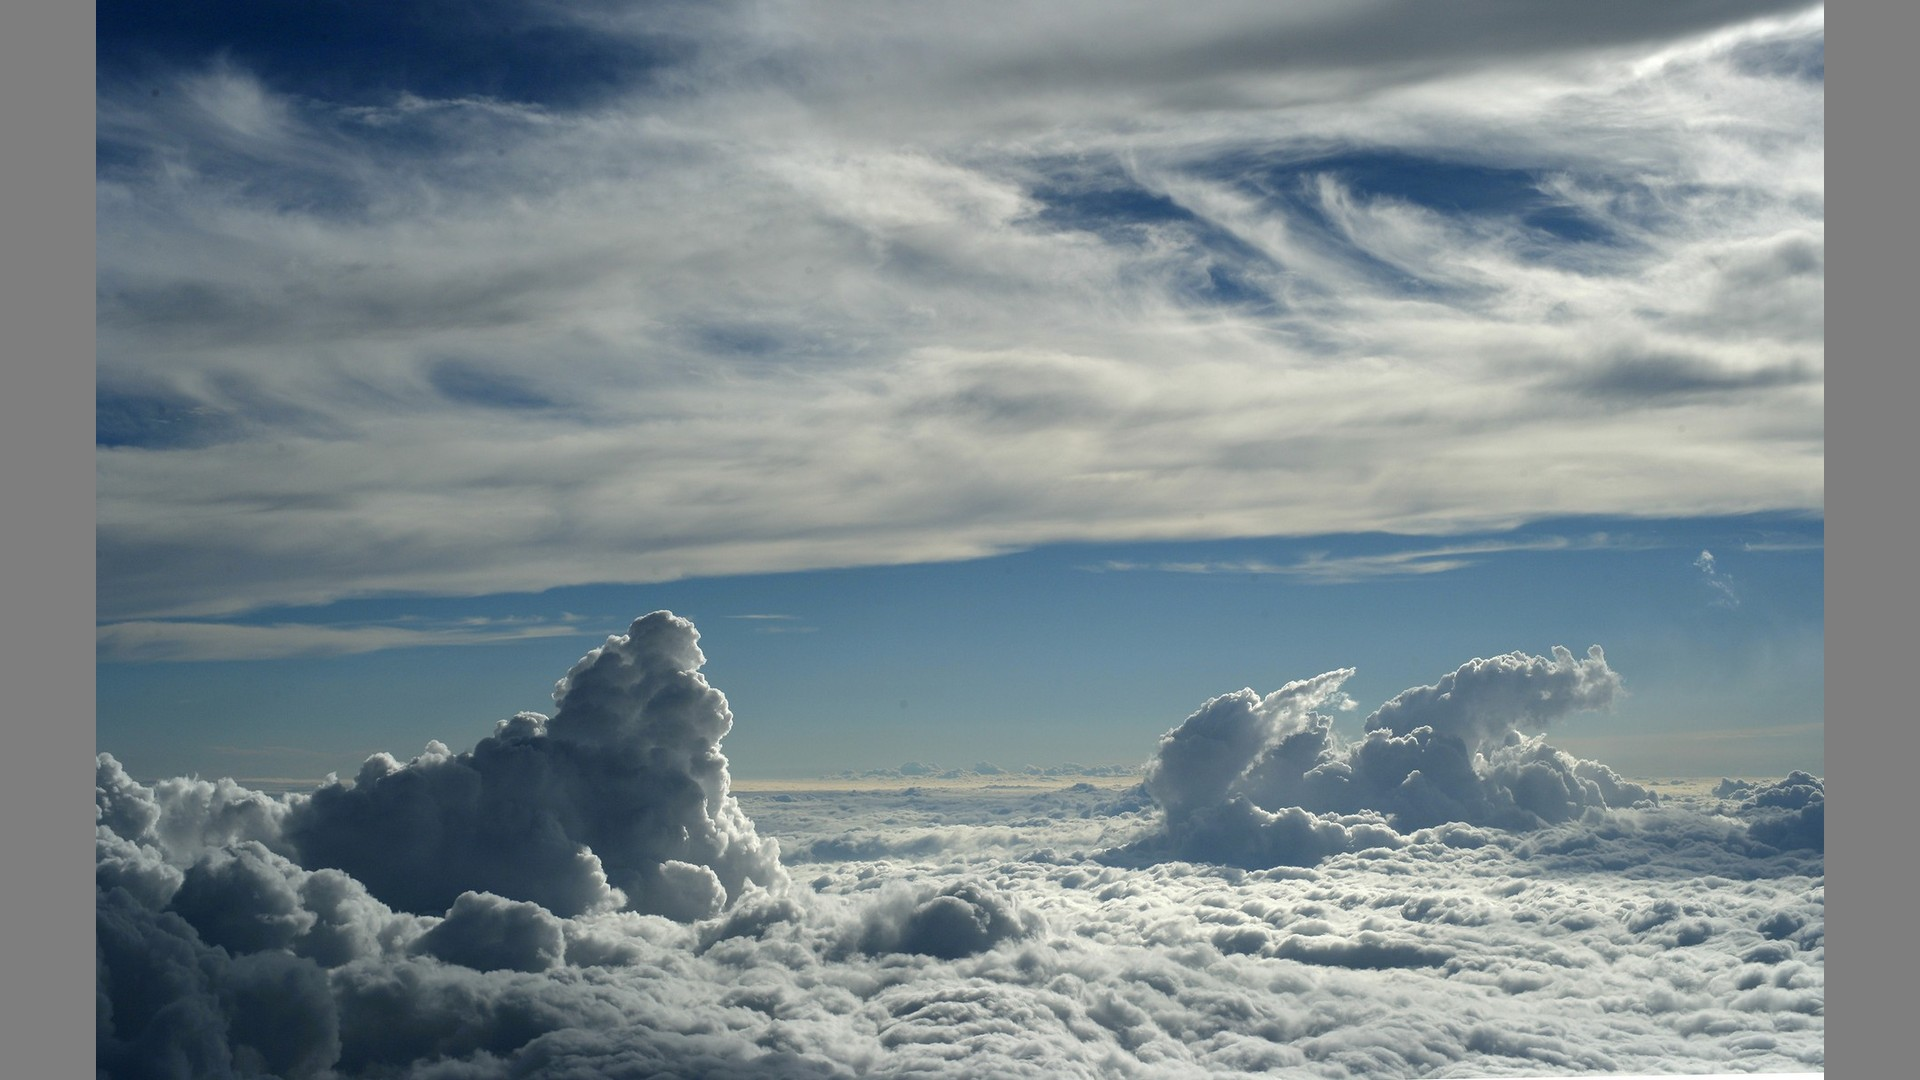
\includegraphics[width=3in]{imgs/example1_original.jpg}}
    \hspace{5mm}
    \subfloat[][Saliency map]{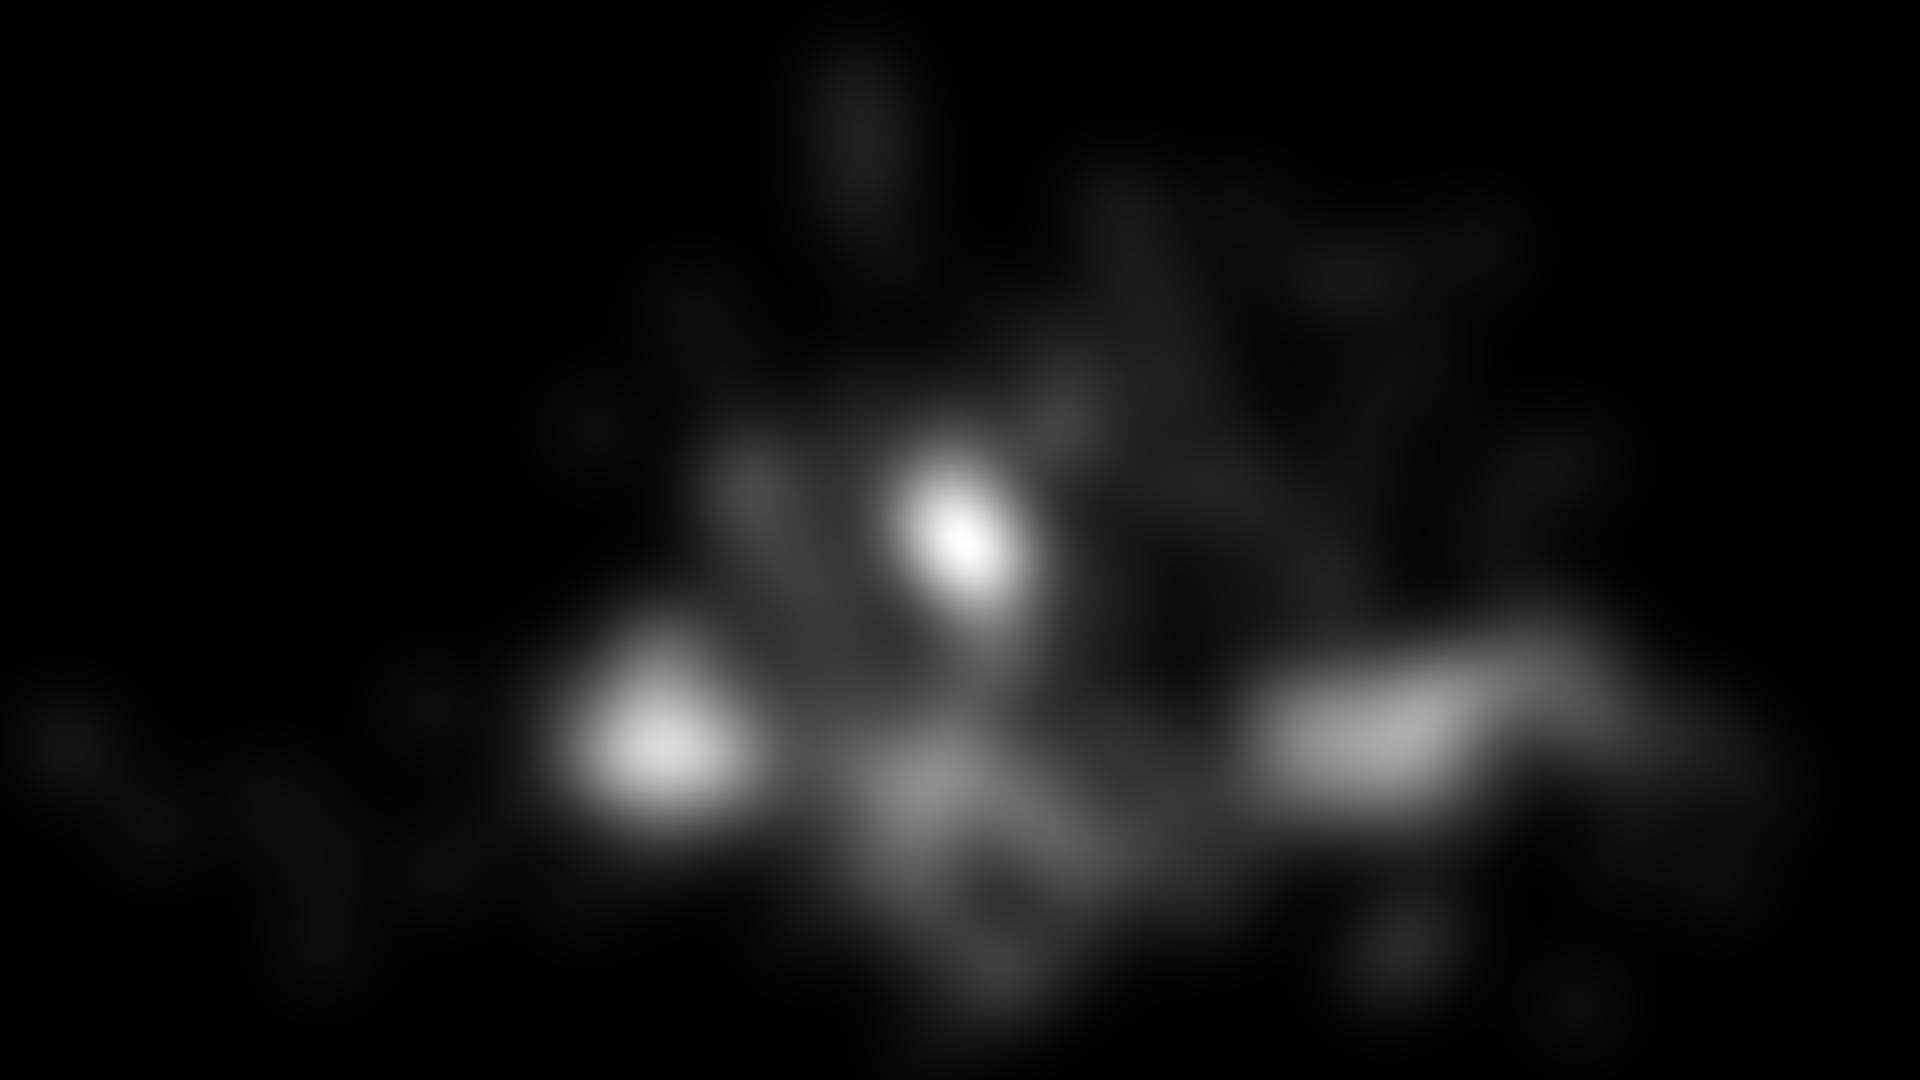
\includegraphics[width=3in]{imgs/example1_saliency.jpg}}
    \caption{Data example}
    \label{img:data_example}
\end{figure}


\section{Related Work}

Visual saliency detection methods can be categorized into bottom-up models and top-down models \cite{congReviewVisualSaliency2019}.
Before deep learning was widely applied in this field, most of the early methods are bottom-up models.
Those early methods usually involve biological and psychological research about visual attention mechanisms. Moreover, those two approaches match the common beliefs about the biological process of human vision.
In general, those models try to establish links between visual saliency and low-level image features, such as color, contrast, brightness, etc. The Itti. model\cite{ittiModelSaliencybasedVisual1998}
is one of the earliest models of this kind, which predicts visual saliency from a linear combination of features calculated from color, intensity, and orientation.
Some other techniques are also used to achieve better results, such as frequency domain analysis, sparse representation, cellular automata, etc. \cite{congReviewVisualSaliency2019}


On the other hand, top-down models try to find what factors have the most impact on visual saliency. Those models use visual saliency datasets-which contain images and their saliency annotations-
to analyze them in a data-driven fashion.
In recent years, deep learning is introduced into this area and has boosted the performance of saliency prediction a lot.
Vig et al. \cite{vigLargeScaleOptimizationHierarchical2014} proposed the first neural network for saliency prediction, combining convolutional neural network (CNN) and support vector machine (SVM). Later, researchers start to use transfer learning for saliency detection tasks. Very Deep Convolutional Networks (VGG) are used in multiple models \cite{kruthiventiDeepFixFullyConvolutional2015, kummererDeepGazeIIReading2016, corniaPredictingHumanEye2018}, and some of them incorporate Gaussian prior for performance improvement.
Generative adversarial networks also achieve good results in saliency prediction \cite{panSalGANVisualSaliency2018, cheHowGazeInfluenced2020}.

Transformers are networks based on attention mechanisms and were first applied in natural language processing (NLP) for their ability to model long-range and multi-level information \cite{bahdanauNeuralMachineTranslation2016a, vaswaniAttentionAllYou2017a}.
They are later introduced for computer vision tasks and show strong potential in modeling non-local dependencies in images \cite{zhangSelfAttentionGenerativeAdversarial2019a}.
However, this technique has not been applied in visual saliency tasks so far.

Our trial of applying attention mechanism to CNNs to improve the performance also has supporting evidence from cognitive psychology. Two contradictory models try to explain the human attention mechanism \cite{gazzaniga2006cognitive}.
In the “Early Selection Model,” a complete analysis is unnecessary for an unimportant stimulus before it is excluded from our focus area. In contrast, in the “Late Selection Model,” all the stimuli are equally processed until they reach at least the semantic level.
Both models have evidence, and the key to solving the divergence is to find the threshold between them. From this view, since CNN usually has small receptive fields in the first few layers, the information is highly abstract for high-level analysis. Hence, traditional models can be regarded as similar to the late selection.
The computer vision attention mechanism focuses more on global information. We guess that its low-level preprocessing can ease the burden of CNN and guide it to a better result.

\section{Data}
\subsection{Datasets}
\label{sec:datasets}
The datasets that are commonly used for image saliency prediction tasks are MIT1003 \cite{judd2012benchmark}, CAT2000 \cite{borji2015cat2000} and SALICON \cite{jiang2015salicon}.
In all three datasets, the original data are normal pictures. Grey margins are attached to some of the pictures to make them the same size. 
The labels, or the training targets, are heatmaps that highlight some interesting regions to humans.
Generally, those datasets are created using eye-tracking devices or mouse tracking software. The trajectories of eye/mouse movement while
observing the test images are recorded, and fixation maps can be created
by placing the trajectories as white pixels on black backgrounds. The fixation maps are \textbf{binary} in a sense that
the pixel values are either $0$ or $255$ in the fixation maps.
Saliency maps are generated by applying a Gaussian filter to the fixation maps and then normalize the results to range $[0, 1]$ (\textbf{continuous values}).
Fig. \ref{img:data_example_2} shows one example from SALICON dataset, of the original image, its corresponding
fixation map, and the saliency map created by applying a Gaussian blur to the fixation map with $\sigma=19$.
\begin{figure}[h!]
    \centering
    \subfloat[][Original]{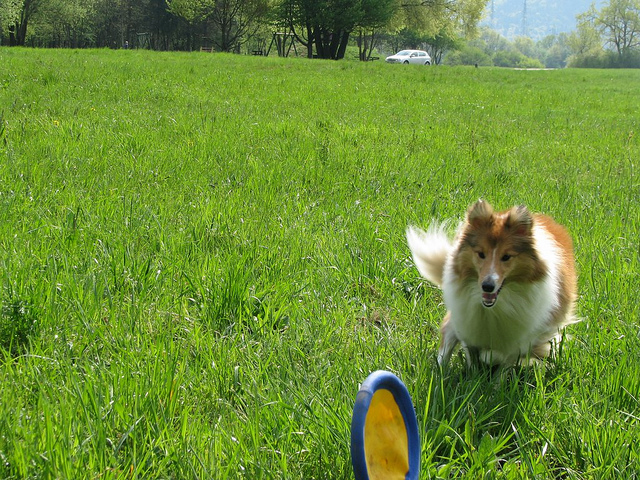
\includegraphics[width=2.5in]{imgs/example2_original.jpg}}
    \hspace{1mm}
    \subfloat[][Fixation map]{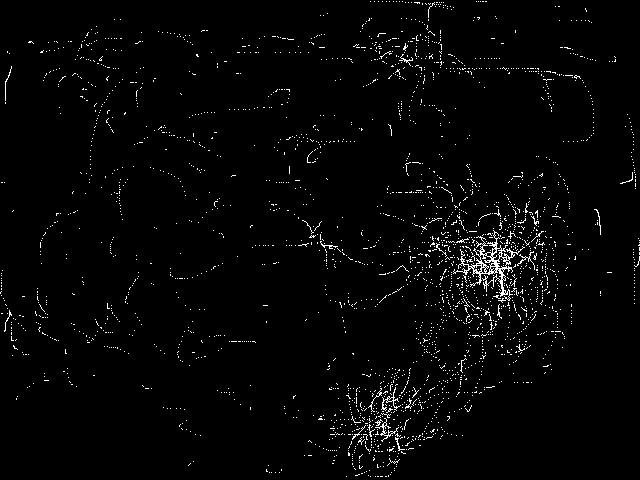
\includegraphics[width=2.5in]{imgs/example2_fixation.png}}
    \hspace{1mm}
    \subfloat[][Saliency map]{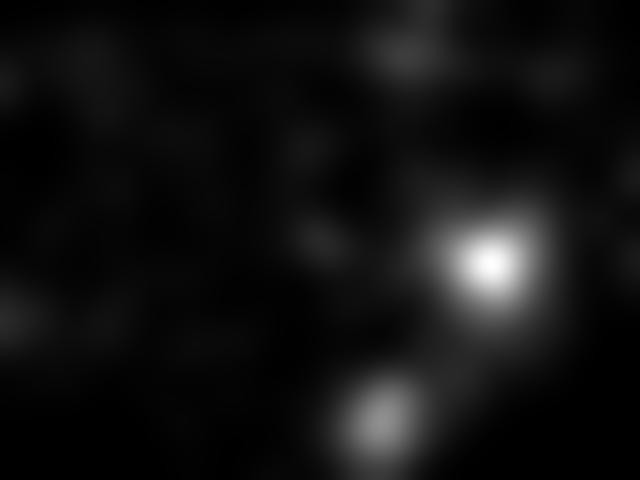
\includegraphics[width=2.5in]{imgs/example2_saliency.jpg}}
    \caption{Data example}
    \label{img:data_example_2}
\end{figure}

The CAT2000 contains 4000 images from 20 different categories. In those images, 2000 are for training and the other 2000
are for testing. There are 24 test subjects for each image and a total of 120 test subjects. The free viewing duration is 5 seconds. Fixation data from only 18 out of 24 test subjects are available in the training
set, and the test set is released with only the original images.

The SALICON dataset is created using images from Microsoft Common Objects in Context (MS COCO) dataset\cite{linMicrosoftCOCOCommon2015}.
Instead of using an eye-tracker, mouse trajectories from different viewers are used in this dataset to calculate the probability distribution of visual attention. A total of 20000 images from 80 categories, including
10000 in the training set, 5000 in the validation set, and 5000 in the test set.
In the training set, the original images, fixation maps, and saliency maps are all available, while
the test set is released without fixation maps and saliency maps.


We plan to combine the training and validation set of SALICON
and split it into ten folds (7 for training, 2 for validation, and 1 for testing).
Our training data are the seven folds from SALICON.
Our validation data for tuning the hyper-parameters are the other two folds from SALICON,
and our testing data consists of the remaining one fold from SALICON together with CAT2000.

Some datasets might not have ground truth saliency maps available, and different datasets might use different Gaussian standard variance to create the saliency maps.
Therefore, we need to generate saliency maps using a set of uniformed parameters from fixation data.

All images are resized to $256 \times 256$ and normalized using mean ($[0.485, 0.456, 0.406]$)and standard deviation ($[0.229, 0.224, 0.225]$).



\subsection{Interpretability}

The visual saliency algorithm takes an input of the original figure and outputs a saliency map of the same size. Each pixel contains a float number from 0 to 1. Bigger numbers show that these pixels or areas get more focus. Therefore, it is a regression task, and the output can be visualized by plotting the saliency map. We can intuitively judge whether the output saliency map corresponds with real data from people to check its interpretability from the visualization.

\begin{itemize}
    \item The deep neural network is compelling and can fit complex functions. If we insert a layer for attention, how should we confirm that adding this layer can effectively improve performance? Other simpler layers cannot replace its function (like fully connection layers) or integrated into other layers?
    \item If the performance is good, how should we learn whether the final result depends largely on the attention layer since its function is to assign some weights to some features?
    \item We previously assume that the attention layers help the network to focus on global information and cooperate with convolutional layers that focus on local features. How can we find evidence for this assumption?
\end{itemize}


\section{Analysis}
\subsection{Algorithm}
We choose CNN to predict the saliency maps. The filters in CNNs function as feature extractors,
and as the depth of the convolutional layer go up, the features tend to be more sophisticated
and high level. If we have learnable parameters assigned to different filters, the model can learn to predict which features are more attractive to humans.
This feature of CNNs fits our need of detecting visual saliency, and it is why we chose CNN.


We use UNet \cite{ronnebergerUNetConvolutionalNetworks2015} as the backbone of our model. UNet has a symmetric expanding path made of several skip connections that enables precise localization. This feature can help assign correct visual saliency values to the corresponding locations. It also enables UNet to incorporate both low-level features and
high-level features. The structure of our model is shown in \ref{img:network}. The numbers under each
module indicate the width of the convolutional layer (number of filters/kernels) and determine the length of each module on the x-axis.
The area of the east/west face indicates
the relative size of the resulting image/feature map of that module.

\begin{figure}[h!]
    \centering
    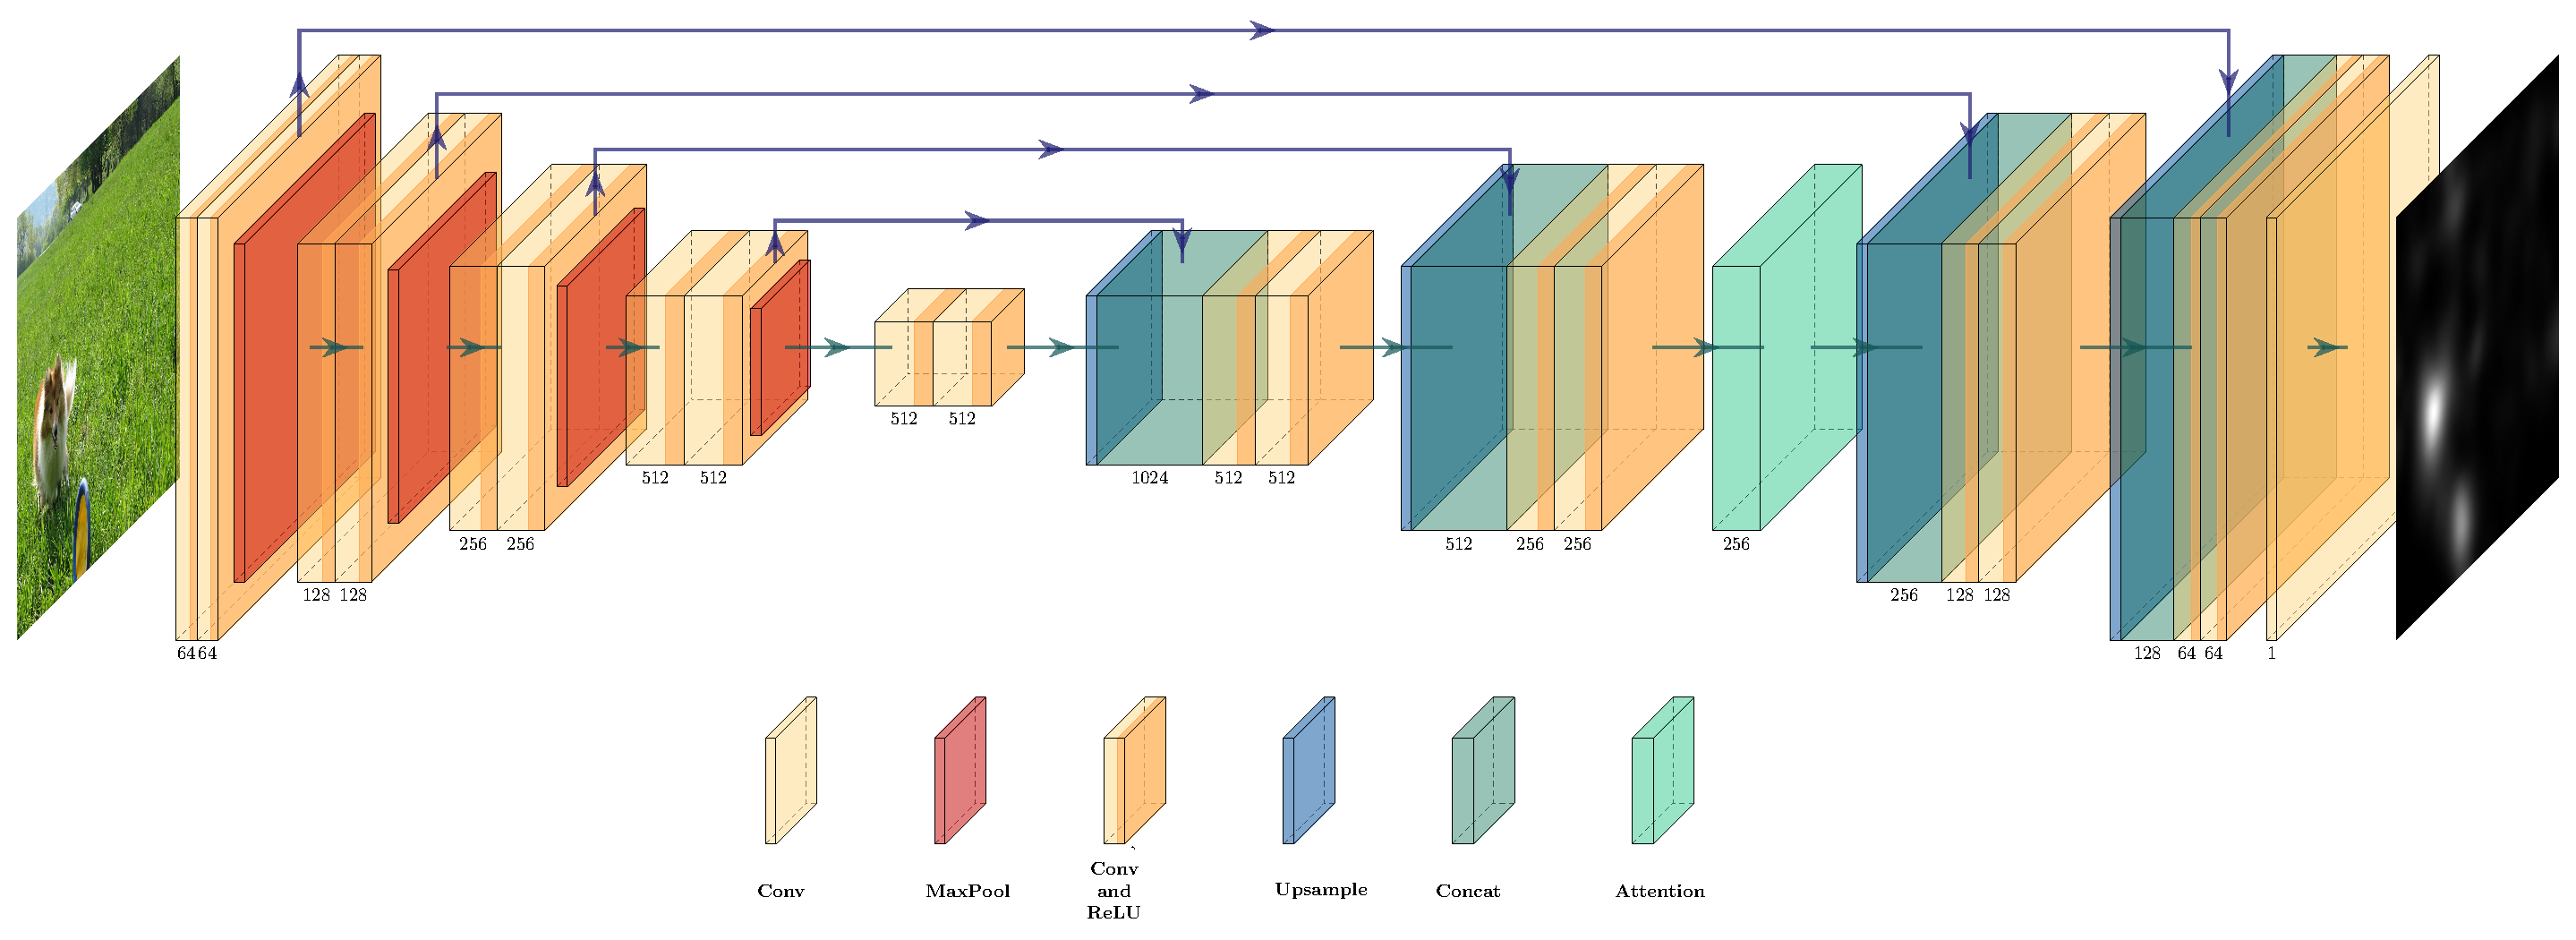
\includegraphics[width=7in]{imgs/network.pdf}
    \caption{Network structure}
    \label{img:network}
\end{figure}

As for the attention mechanism, we implement it as a Pytorch module and then make this module
part of UNet's data path. The goal of this module is to find long-distance dependencies across different parts in the image. The reason for introducing this module is that CNNs have a limited
reception field decided by the sizes of convolutional kernels, and we hope to alleviate this problem
by using attention mechanisms. We use the similar attention module described in
\cite{zhangSelfAttentionGenerativeAdversarial2019a}, and the structure of the attention module is shown in
\ref{img:attention}. The attention map is a $1 \times N \times N$ tensor, where $N$ is the total number of
pixels in the output of $f(x)$ (or $g(x)$, they output tensors of the same size). This map acts like a
relationship matrix, where each element in the matrix indicates the bond/dependency between two particular
pixels in the input feature map. However, applying this attention module directly to the original input
image will result in a huge attention map which would consume a lot of memory and make the calculations
expensive. Therefore we put this module in the middle part of the network, where the feature map is relatively
small. We also reduced the number of kernels of $f(x)$, $g(x)$, and $h(x)$ to further reduce the memory
usage and speed up the execution.

\begin{figure}[h!]
    \centering
    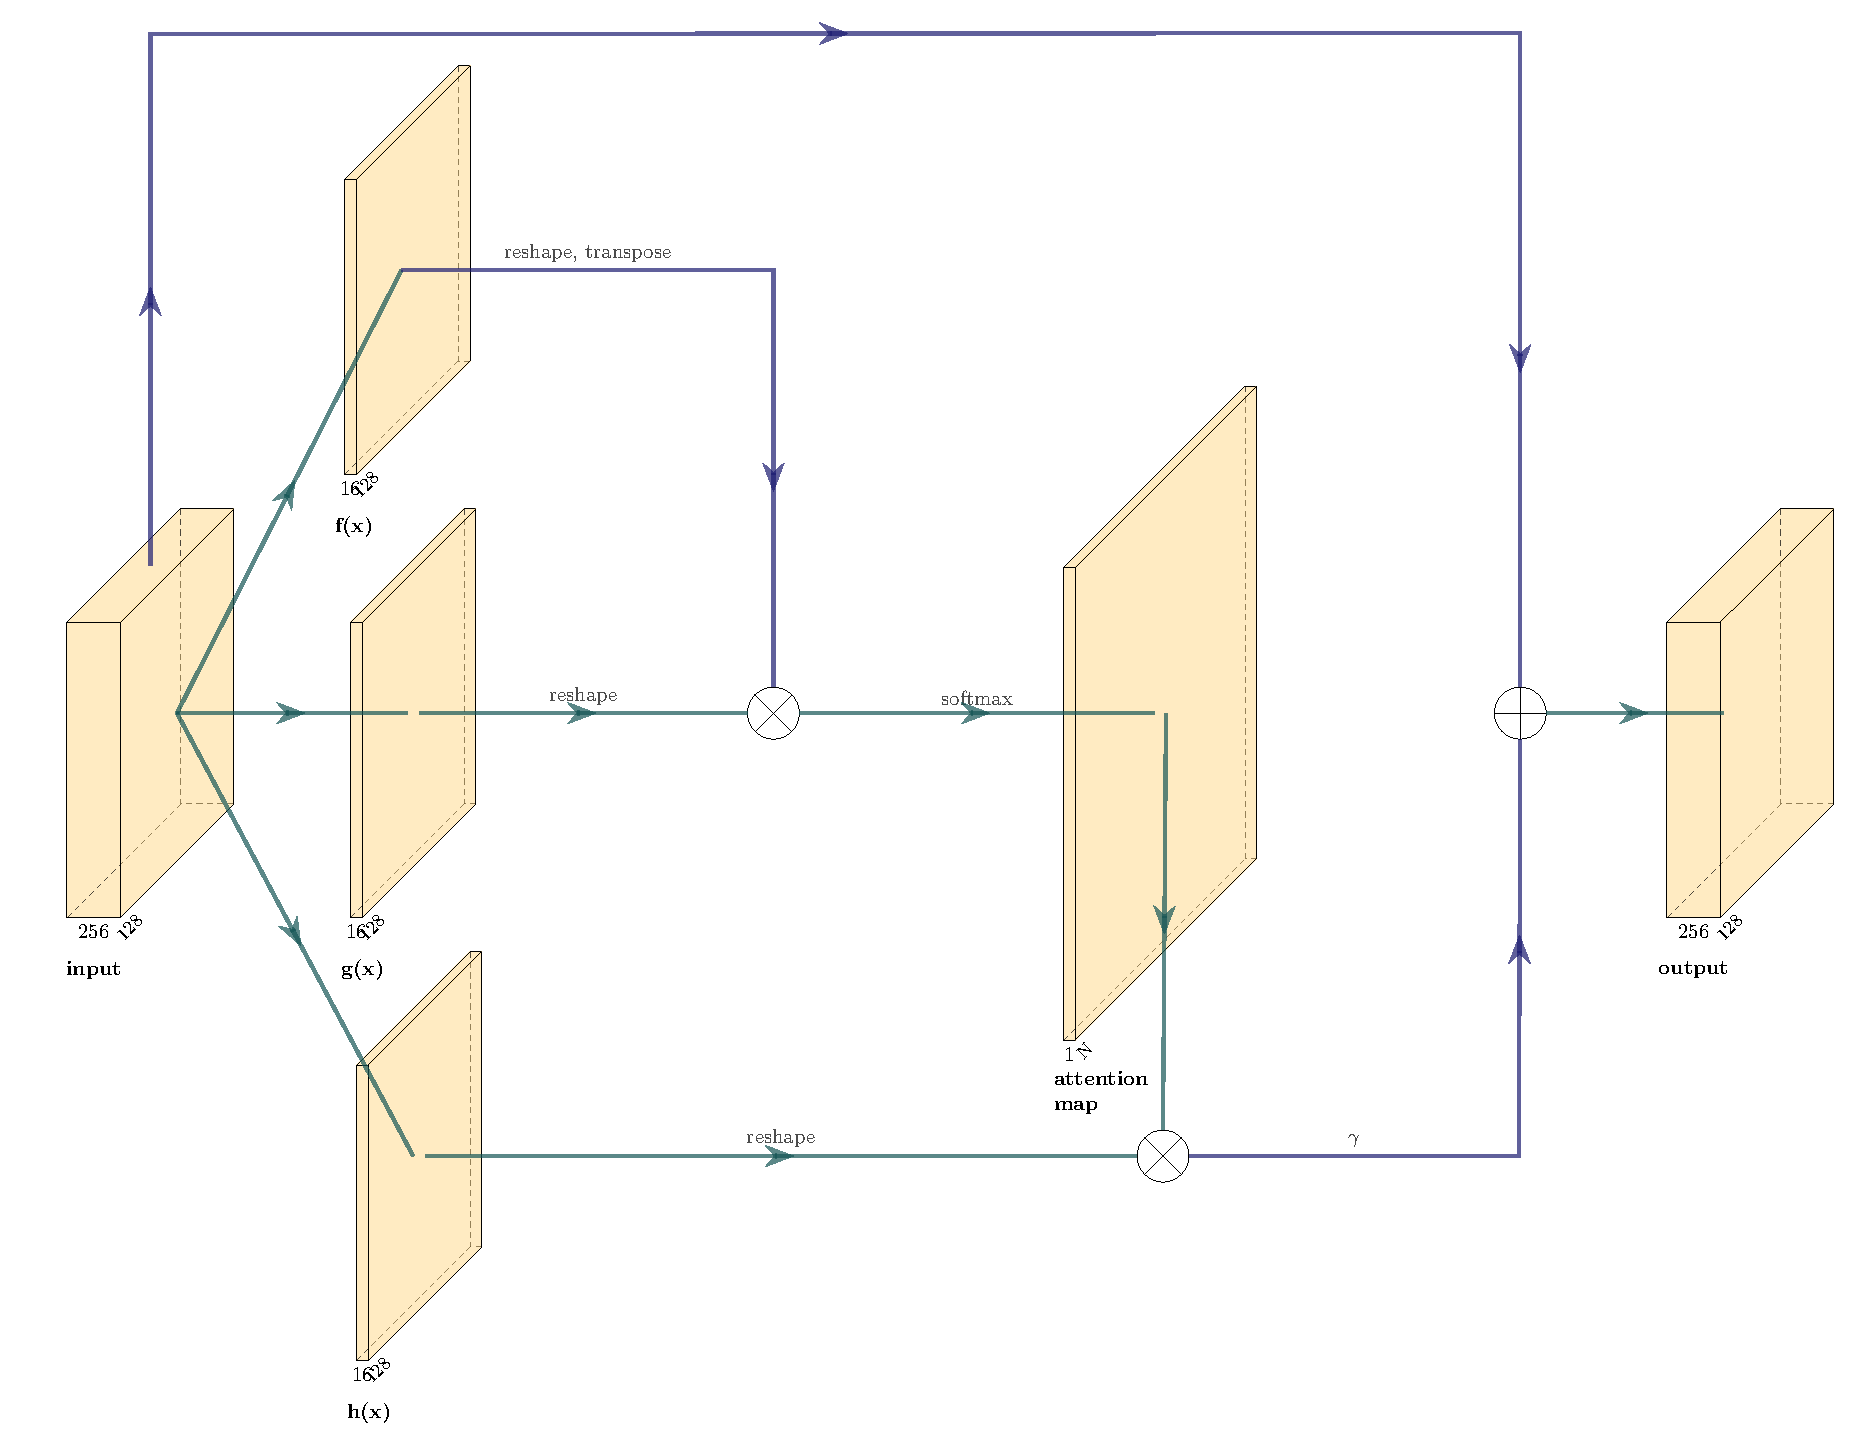
\includegraphics[width=4in]{imgs/attention.pdf}
    \caption{Attention module structure}
    \label{img:attention}
\end{figure}


Considering this is an end-to-end model, the dataflow will be pretty straightforward. The input data is fed to the model,
and then the output is compared with ground truth to compute the loss. The loss is then backpropagated to update model parameters.

Since the test sets' ground truths of these datasets are not public, we will divide the original dataset into the train set, the validation set, and the test set. We can choose suitable hyper-parameters based on the results of the train set and the validation set.

\subsection{Performance Measurement}

There are several metrics that can be used to measure the performance. According to \cite{riche2013saliency}, these various metrics may reflect different properties of the algorithm.
\begin{itemize}
    \item Normalized scanpath saliency (NSS \cite{petersComponentsBottomupGaze2005})
    \item Correlation coefficient (CC)
    \item Area under receiver operating characteristic curve(AUC \cite{richeSaliencyHumanFixations2013})
    \item etc.
\end{itemize}

The NSS measures the mean saliency value at fixated locations of the normalized (zero mean, unit variance) saliency map. 
It can be calculated using Eq. \ref{EQ:NSS}. 
\begin{equation}
    \begin{aligned}
        NSS &= \frac{\sum^{N} T_{i}}{N}\\
        \text{where }T &= \frac{S - \bar{S}}{\sigma_{S}} \circ F
    \end{aligned}
    \label{EQ:NSS}
\end{equation}
In this equation, $S$ is the saliency map, $\bar{S}$ is the mean of $S$, $\sigma_{S}$ is 
the standard deviation of $S$, $F$ is the fixation map with only $0$ and $1$ as pixel values in it,
$T_{i}$ is the pixel value in $T$ at location $i$, and $N$ is the total number of non-zero pixels in $F$.
One way to interprete it is that it represents the confidence interval $(-NSS\times\sigma, NSS\times\sigma)$, where
$\sigma = 1$. Therefore a higher NSS means a larger confidence interval, i.e. better performance.

The CC is the linear correlation coefficient between a model saliency map and an empirical saliency map gained from convolving the fixation locations with a Gaussian kernel.
It can be calculated using EQ. \ref{EQ:CC}.
\begin{equation}
    \begin{aligned}
        CC = \frac{\sum_{i=1}^{n}(x_{i}-\bar{x})(y_{i}-\bar{y})}
        {\sqrt{\sum_{i=1}^{n}(x_{i}-\bar{x})^{2}}\sqrt{\sum_{i=1}^{n}(y_{i}-\bar{y})^{2}}}
    \end{aligned}
    \label{EQ:CC}
\end{equation}


In AUC metric,
the saliency map is treated as a binary classifier to separate positive from negative samples at various thresholds. 
The true positive (TP) rate is the proportion of saliency map values above the threshold at fixation locations.
The false positive (FP) rate is the proportion of saliency map values above the threshold at all pixels.
We calculate the TP rate and FP rate using a series of thresholds between $[0, 1]$, and draw a
receiver operating characteristic (ROC) curve with FP rate as x-axis and TP rate as y-axis.
An example of this curve is shown in Fig. \ref{img:AUC} \cite{hanleyMeaningUseArea1982}.
The area under this curve is reported as AUC.

\begin{figure}[h!]
    \centering
    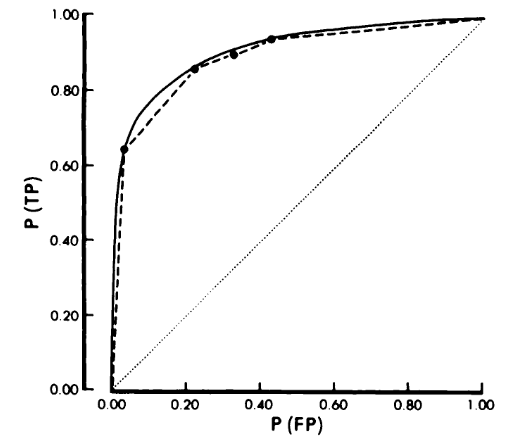
\includegraphics[width=2.5in]{imgs/AUC.png}
    \caption{ROC curve example\cite{hanleyMeaningUseArea1982}}
    \label{img:AUC}
\end{figure}


The performance is reported on the testing fold of SALICON and also the whole CAT2000 dataset.
Reporting scores using different datasets can make the results more convincing,
because it can show that our model can generalize well.

\subsection{Hyperparameters}
The hyper-parameters that need to be tuned are:
\begin{itemize}
    \item loss function to use,
    \item learning rate.
\end{itemize}

The loss functions we experimented with are:
\begin{itemize}
    \item mean square error (MSE),
    \item NSS,
    \item CC.
\end{itemize}
For learning rate we experimented with $0.01$ and $0.001$.

\section{Results}
% % % Modified by Linsage:Add subtitle begin
\subsection{Model Performance}
% % % Modified by Linsage: Add subtitle end
We use Pytorch Lightning framework \cite{falcon2019pytorch} to implement our project. Our code (including \LaTeX files for this
report) is available at \href{https://github.com/Freddiechang/CMPUT566}{our GitHub repo page}.
The model is trained for 200 epochs under each hyperparameter setting. The performance scores are listed in Table \ref{tbl:performance}.
% % % Modified by Linsage: Add rows and columns begin
\begin{table}[h!]
    \begin{adjustwidth}{-2cm}{0cm}
    \begin{tabular}{ccc|cccc}
        \hline
	   Loss function & $\text{Attention}^{[1]}$ & $\text{Attention}^{[2]}$ & NSS(SALICON) & CC(SALICON) & NSS(CAT2000) & CC(CAT2000)\\
        MSE(3) & Yes & Yes & 1.1585 & 0.8514 & 1.5873 & 0.6063\\
        MSE(3) & Yes & No & 1.1585 & 0.8516 & 1.5878 & 0.6066\\
        MSE(2) & No & No & 1.1639 & 0.8564 & 1.5980 & 0.6102\\
        CC(2) & Yes & Yes & 1.1595 & 0.8533 & 1.5896 & 0.6085\\
        $\text{CC}^{\star}\text{(2)}$& Yes & Yes & 1.1761 & 0.8647 & 1.5989 & 0.6124\\
        $\text{CC}^{\star}\text{(2)}$& Yes & No & 1.1608 & 0.8602 & 1.5748 & 0.6055\\
        CC(1) & No & No & 1.1725 & 0.8624 & 1.6169 & 0.6185\\
        NSS(1) & Yes & Yes & 0.8871 & 0.5984 & 1.2306 & 0.4399\\
        \hline
        \multicolumn{3}{c}{SALICON average} & 1.5691 & 1 & NA & NA \\
        \multicolumn{3}{c}{CAT2000 average} & NA & NA & 2.97 & 1 \\
        \hline
    \end{tabular}
    \end{adjustwidth}
    \caption{Performance under different settings. The numbers in the brackets after the loss function names indicate
how many experiments we did under this setting, and the average performance is reported. We also calculated the performance
baseline using the ground truth fixation maps and saliency maps from the datasets, and the scores are reported in ``SALICON average''
and ``CAT2000 average'' rows. The models with a star sign ($\star$) in their names are trained using a learning rate $0.001$, all
other models are trained using a learning rate $0.01$. ``$\text{Attention}^{[1]}$'' column indicates if the models are trained with attention modules
in them; ``$\text{Attention}^{[2]}$'' column indicates if the attention modules are enabled during test time. }
    \label{tbl:performance}
\end{table}
% % % Modified by Linsage: Add rows and columns end
The model trained using CC, and a learning rate of $0.001$ has the best performance, but the performance
across different hyperparameter settings does not show too much difference. We noticed that
the model performs better on SALICON than on CAT2000. We think the reason for that is the $\sigma$
we used to create the ground truth saliency maps in SALICON is too large. As shown in Table \ref{tbl:performance},
the average NSS for the ground truth saliency maps in SALICON is only $1.5691$, much less than that
of CAT2000. This indicates the highlighted areas in the saliency maps are too large. As a consequence,
the models trained using those saliency maps are not optimal.

Some output examples are shown in Figure \ref{img:output_example}. The model we used to generate those images is trained using CC and a learning rate of $0.001$. The predictions appear to be
very similar to the ground truth, which means our model can successfully determine the visual saliency
in the input images.

\begin{figure}[h!]
    \begin{adjustwidth}{-0.6cm}{}
    \centering
    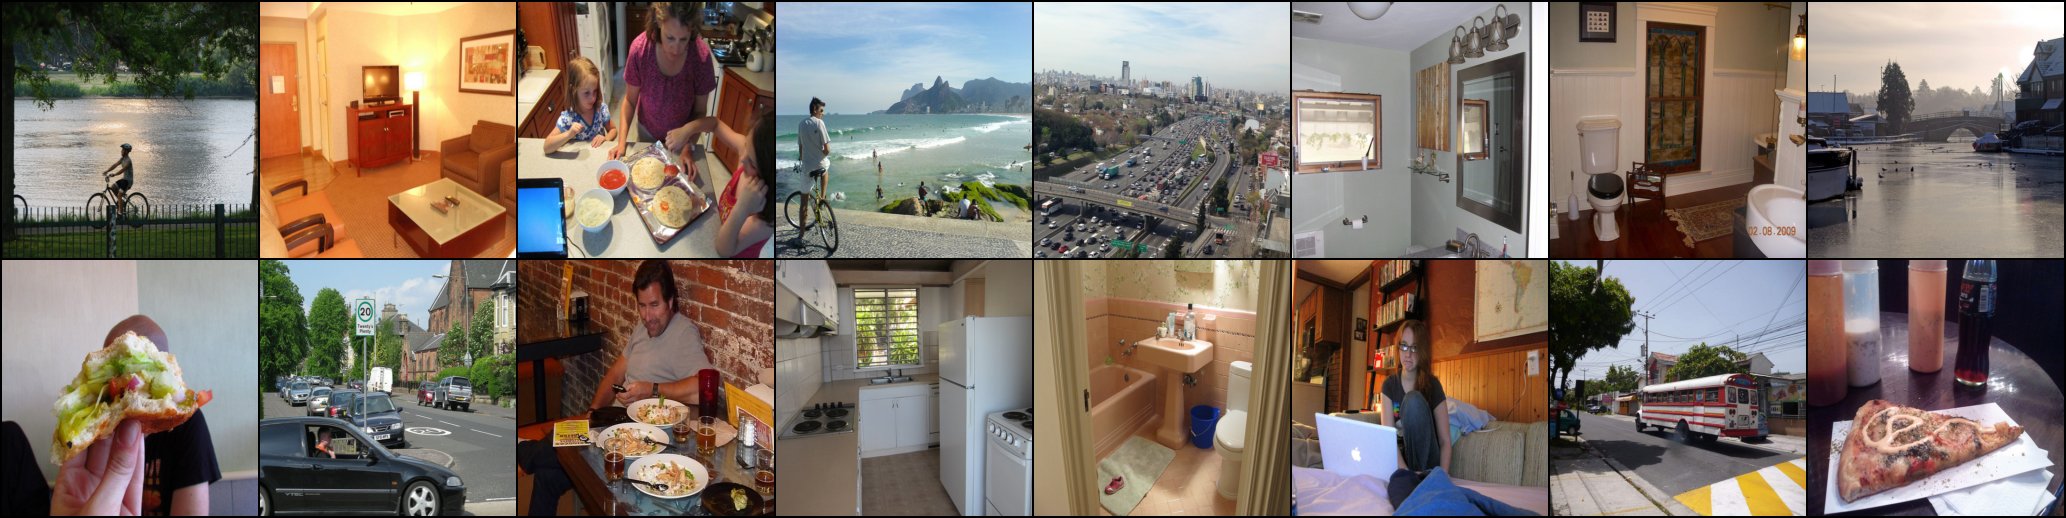
\includegraphics[width=7in]{imgs/out_original_image.png}
    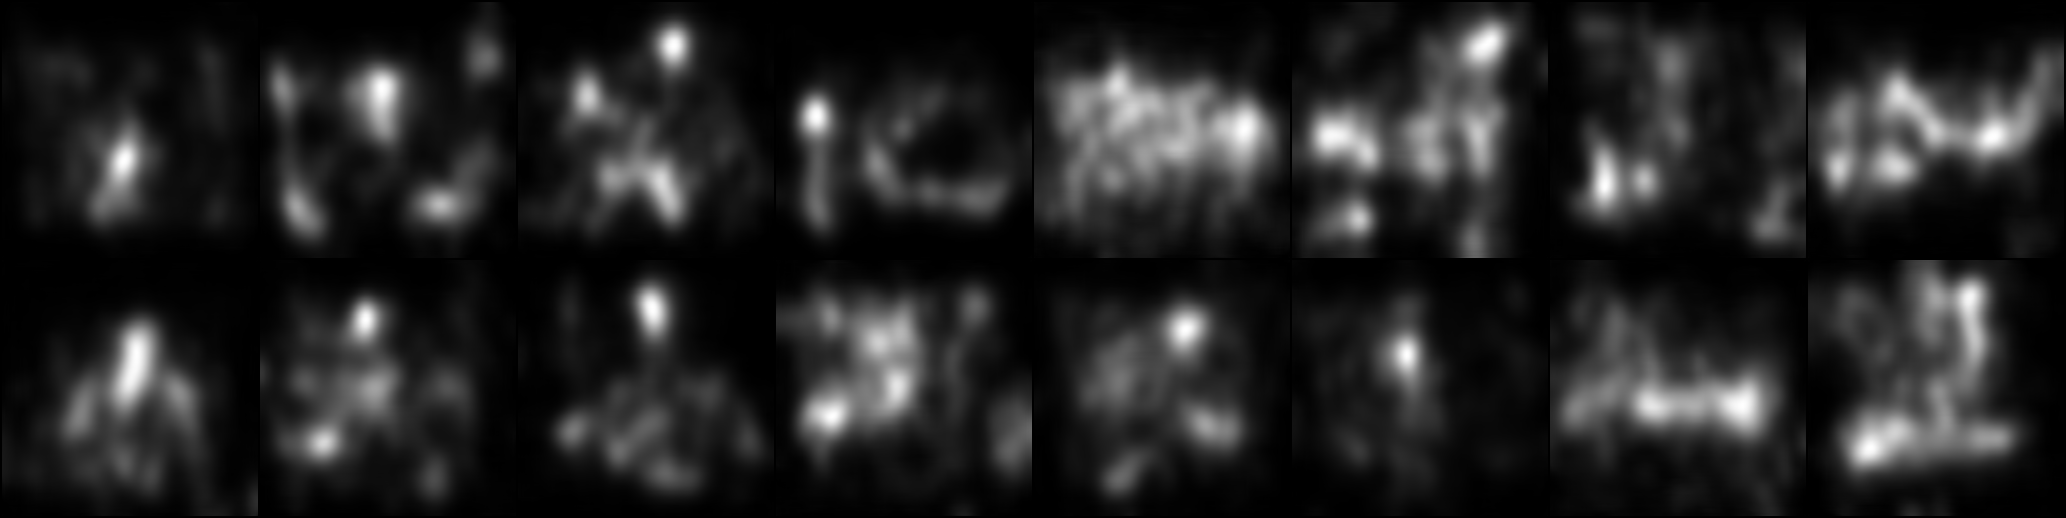
\includegraphics[width=7in]{imgs/out_prediction.png}
    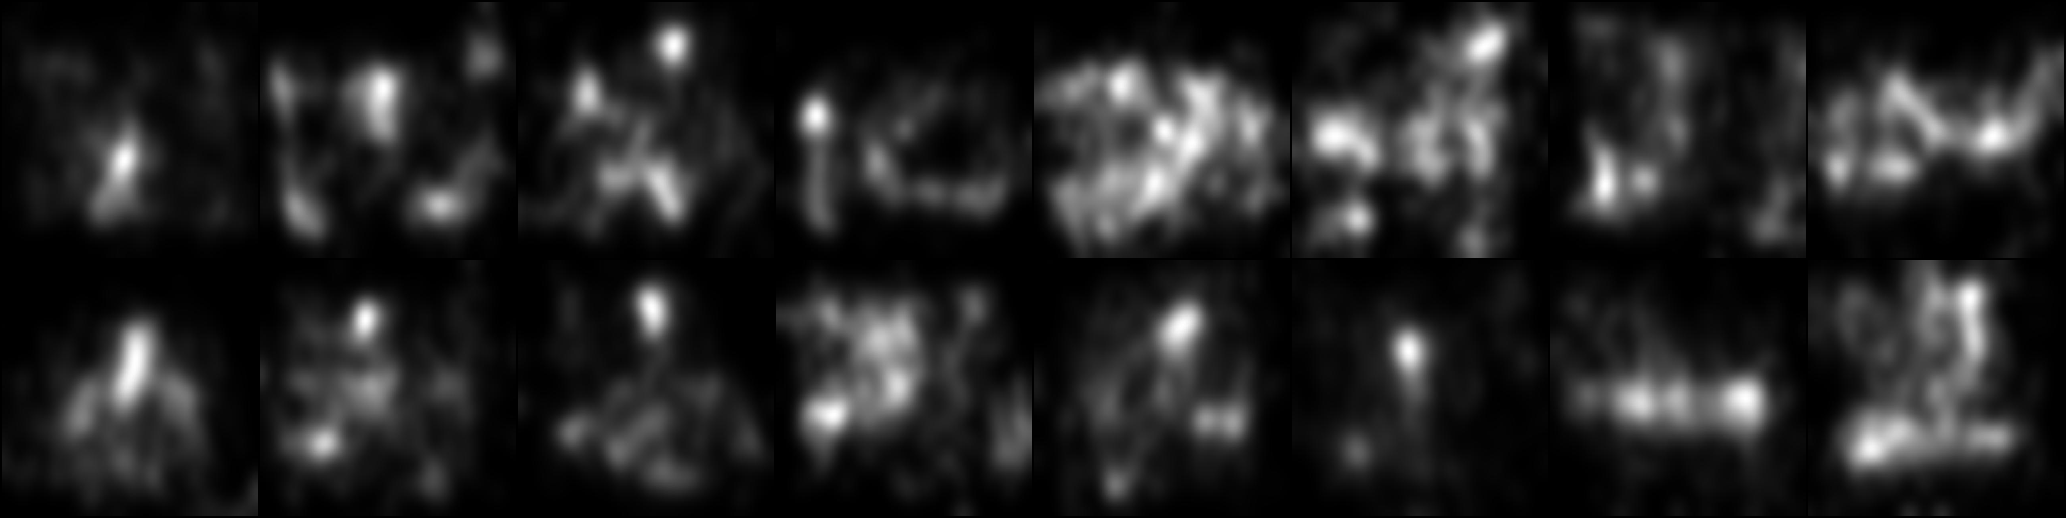
\includegraphics[width=7in]{imgs/out_groundtruth.png}
    \end{adjustwidth}
    \caption{Some output examples. The first two rows are the original input images.
    The second two rows are the predictions of the model. The third two rows are the
    ground truth saliency maps from the SALICON dataset.}
    \label{img:output_example}
\end{figure}
% % % Modified by Linsage: Add Verification and Interpretation begin

The model trained with NSS loss has a performance that is significantly worse than other models.
After we check the outputs, we found that there are many small highlighted spots in the outputs, similar to the fixation map in Figure \ref{img:data_example_2}.
This shows that the model can learn how to produce a fixation map, but the saliency map derived from it does not have the same distribution as the saliency map in the ground truth.

Although the model is trained with SALICON, we also test it on CAT2000, which is an unseen dataset for the model.
We notice that our models achieve NSS > 1.58 and CC > 0.6, which means that these models have good generalizations.
The performance is worse, probably because of two reasons.
SALICON fixation is produced by internet collection of mouse clicking while CAT2000 is derived directly from eye-tracking data.
Almost all the SALICON figures are normal figures which can be categorized by object names (like chair or dog), while CAT2000 contains a large number of specifically designed figures like fractals or stick drawings.


\subsection{Interpretation and Verification}

We use two methods to check the impact of the attention layer.

The first verification is the pre-training modification. We use the same series of training samples to train two models. One of them is with the attention layer. Our networks with the attention layer are sometimes unstable during training and suffer a serious drop in performance.
The training results between the model with and without an attention layer do not have a significant difference.
We suppose that this is because our original UNet is too complicated and redundant, so adding another simple unit cannot help improve the performance. The disturbed training can probably due to a contradiction in training goals between CNN and the attention layer.

The second verification is post-training verification. Namely, during a test, we disable the attention layer to test the result. In the network trained by CC, the performance drops a little, but as a whole, there is not much difference.
When we analyze the output, we found that disabling the attention layer can only make big changes on only a very small portion of pixels and the total change is nearly invisible from visualization.
We suppose that the attention layer can change the weight distribution in the middle of the network. However, due to the complexity of the following layers, its impacts are excessively dispersed, so it does not make conspicuous changes to the output saliency map.

To find some advantage of our network with the attention layer, we browse the outputs of these networks to look for some occasional obvious differences in results.
We mainly search in CAT2000 because it contains more unconventional figures and can inspire how the model is generalized what information the model uses to compute the results.
We use Integrated Gradients \cite{sundararajan2017axiomatic} as the attribution method. We select all the pixels with saliency bigger than threshold = 0.5 and calculate the pixels in the input figures that contribute to their values during the implementation.

Two examples are Figure \ref{img:int_example_1} and Figure \ref{img:int_example_2}, which show that our model may have some ability to capture some global information.

In Figure \ref{img:int_example_1}, the main character is in a very dark color, and the background has some colorful patterns, which attracts the model without the attention layer. The Integrated Gradients figure shows that it is using mainly irrelevant information.
However, the predicted saliency map by the model with the attention layer is almost correct.
From the Integrated Gradients figure, we see that the human body is strongly highlighted. Besides, we find that the pixels which show the margin around the legs also contribute to the result.

Figure \ref{img:int_example_2} is mainly random noise with a obscure stick on the edge. Both models correctly predict that people will mainly focus on the center while our model also finds the stick.
The Integrated Gradients figure also has deeper color in the upper part of the figure than in the lower part. We infer that it is not the stick itself (not highlighted) but the global information in the upper part that helps the decision of saliency map.


\begin{figure}[h!]
    \centering
    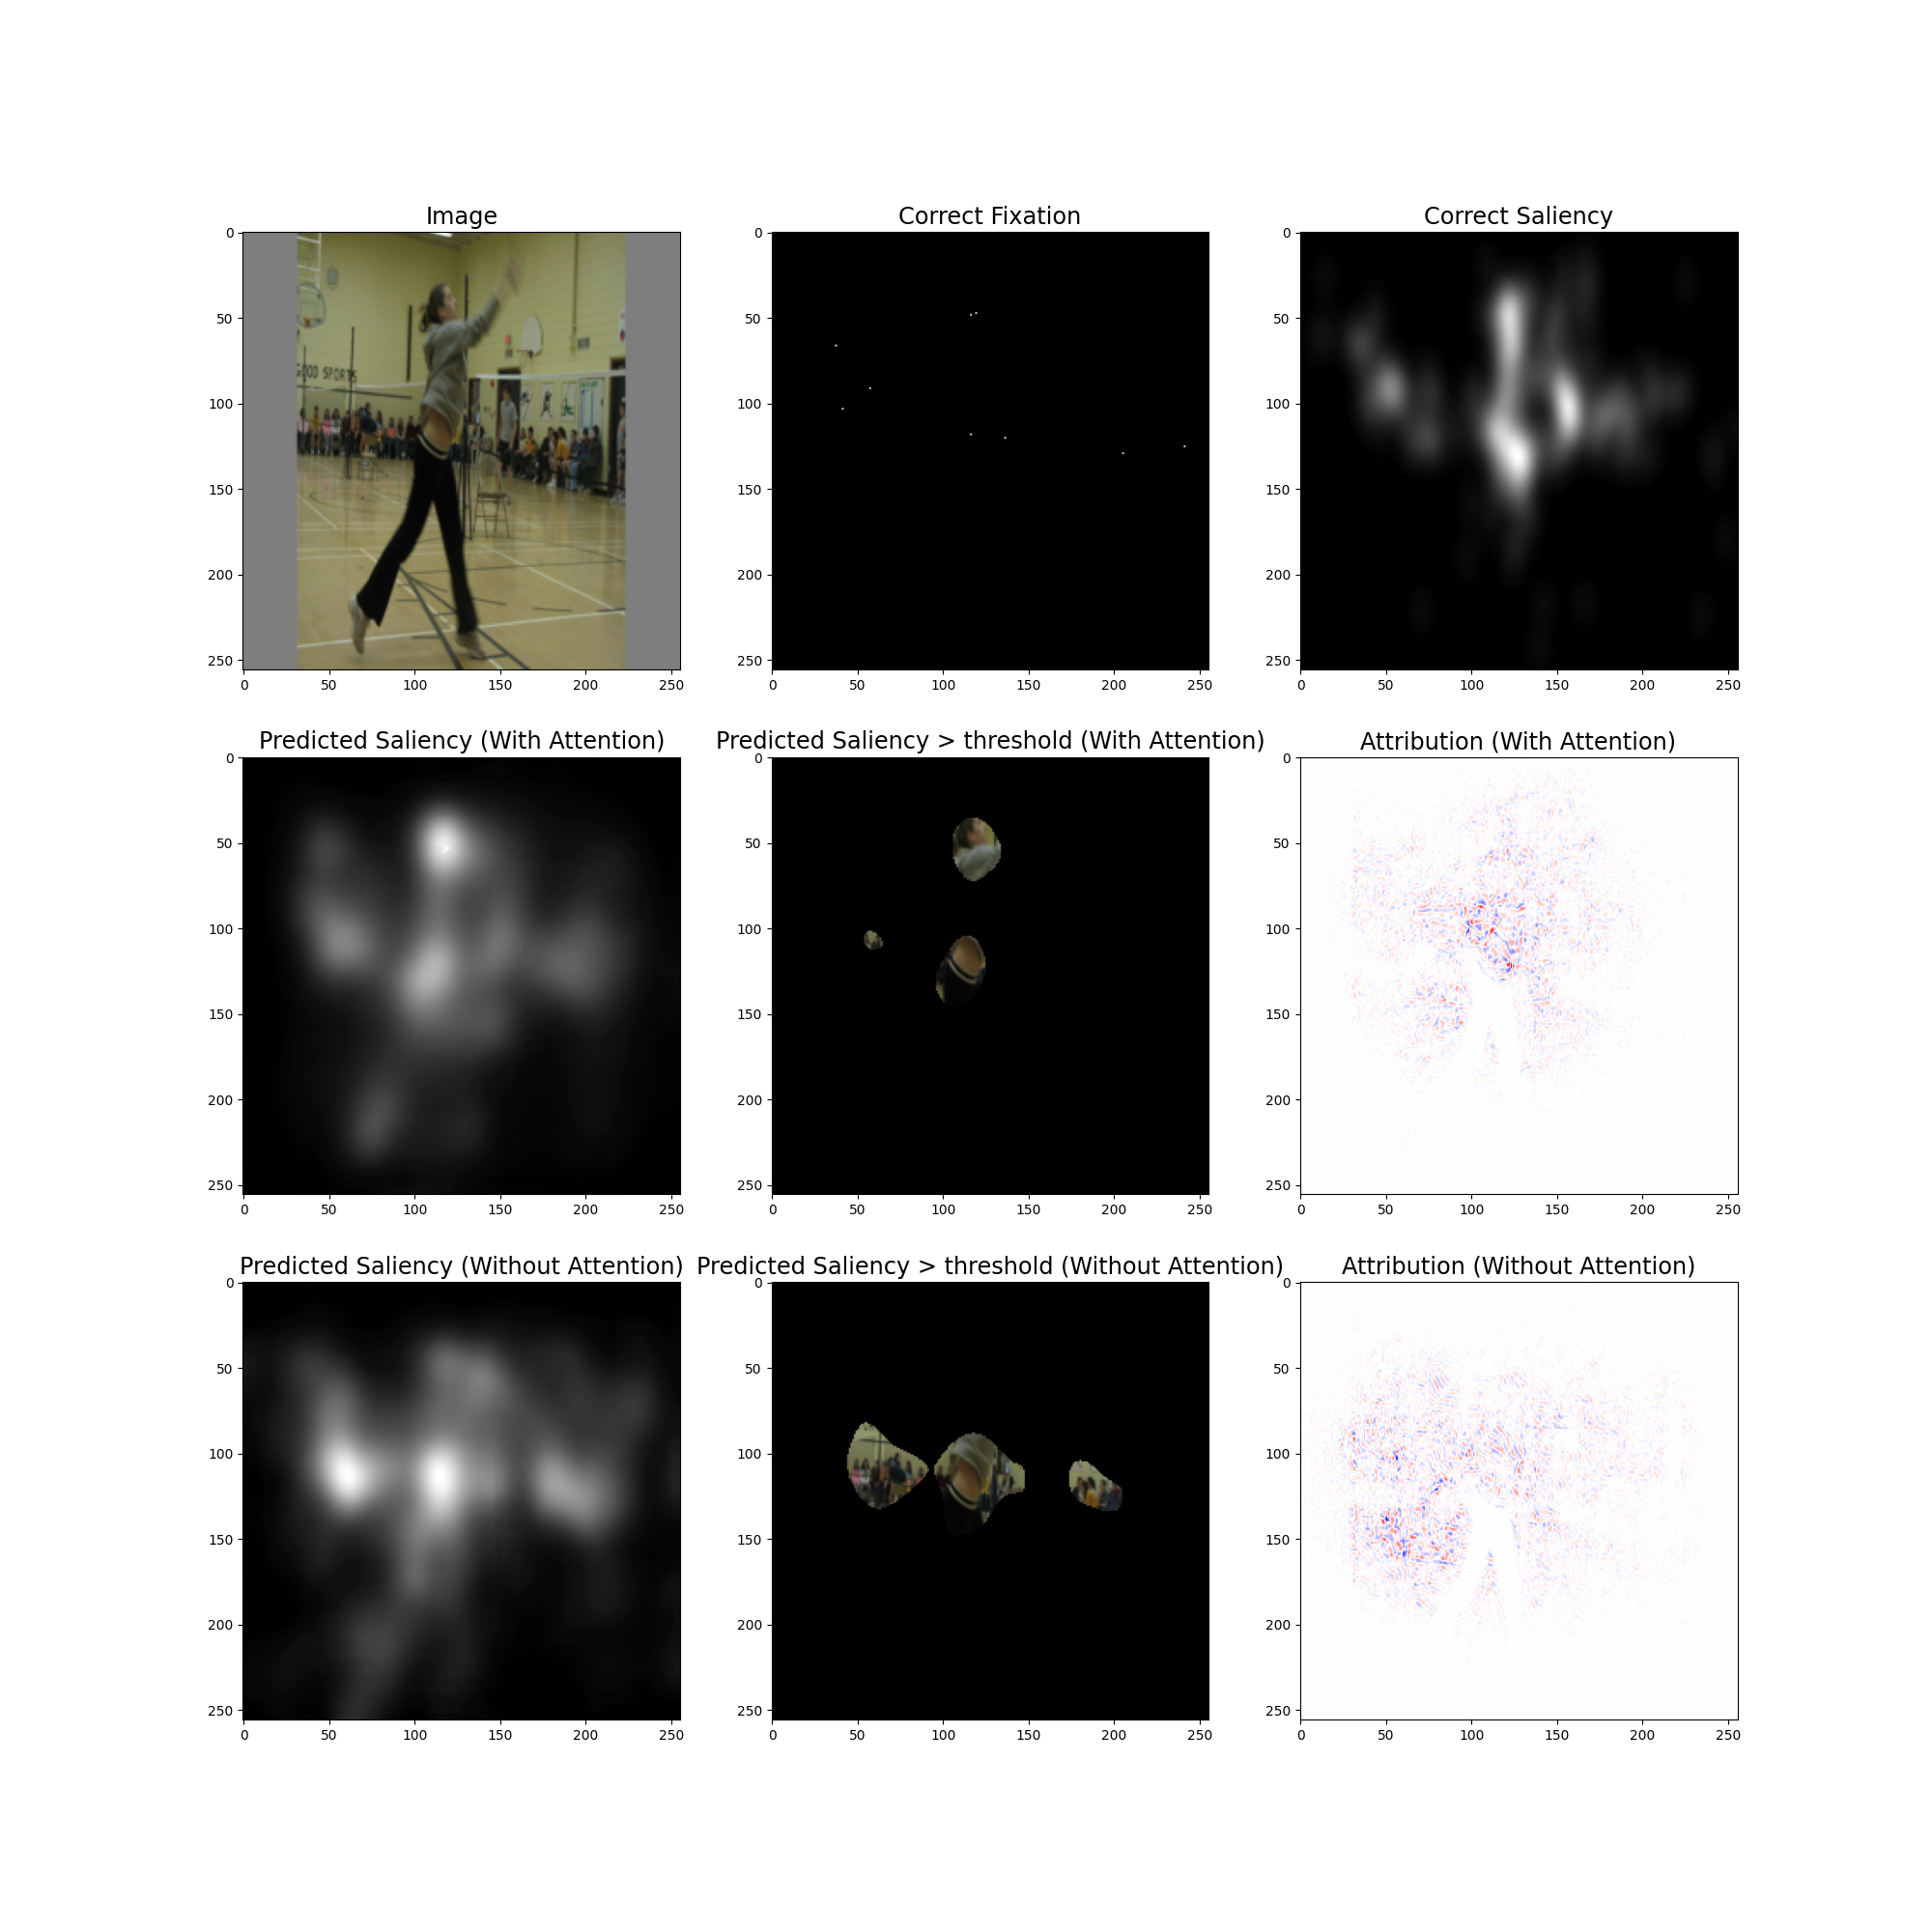
\includegraphics[width=7in]{imgs/used_example_1.png}
    \caption{A figure in Category ``Action'' of CAT2000, the background of which is more colorful than the foreground. The model without attention is led away by human clothes and faces in the background while the model with attention fixes correctly on the main character.}
    \label{img:int_example_1}
\end{figure}

\begin{figure}[h!]
    \centering
    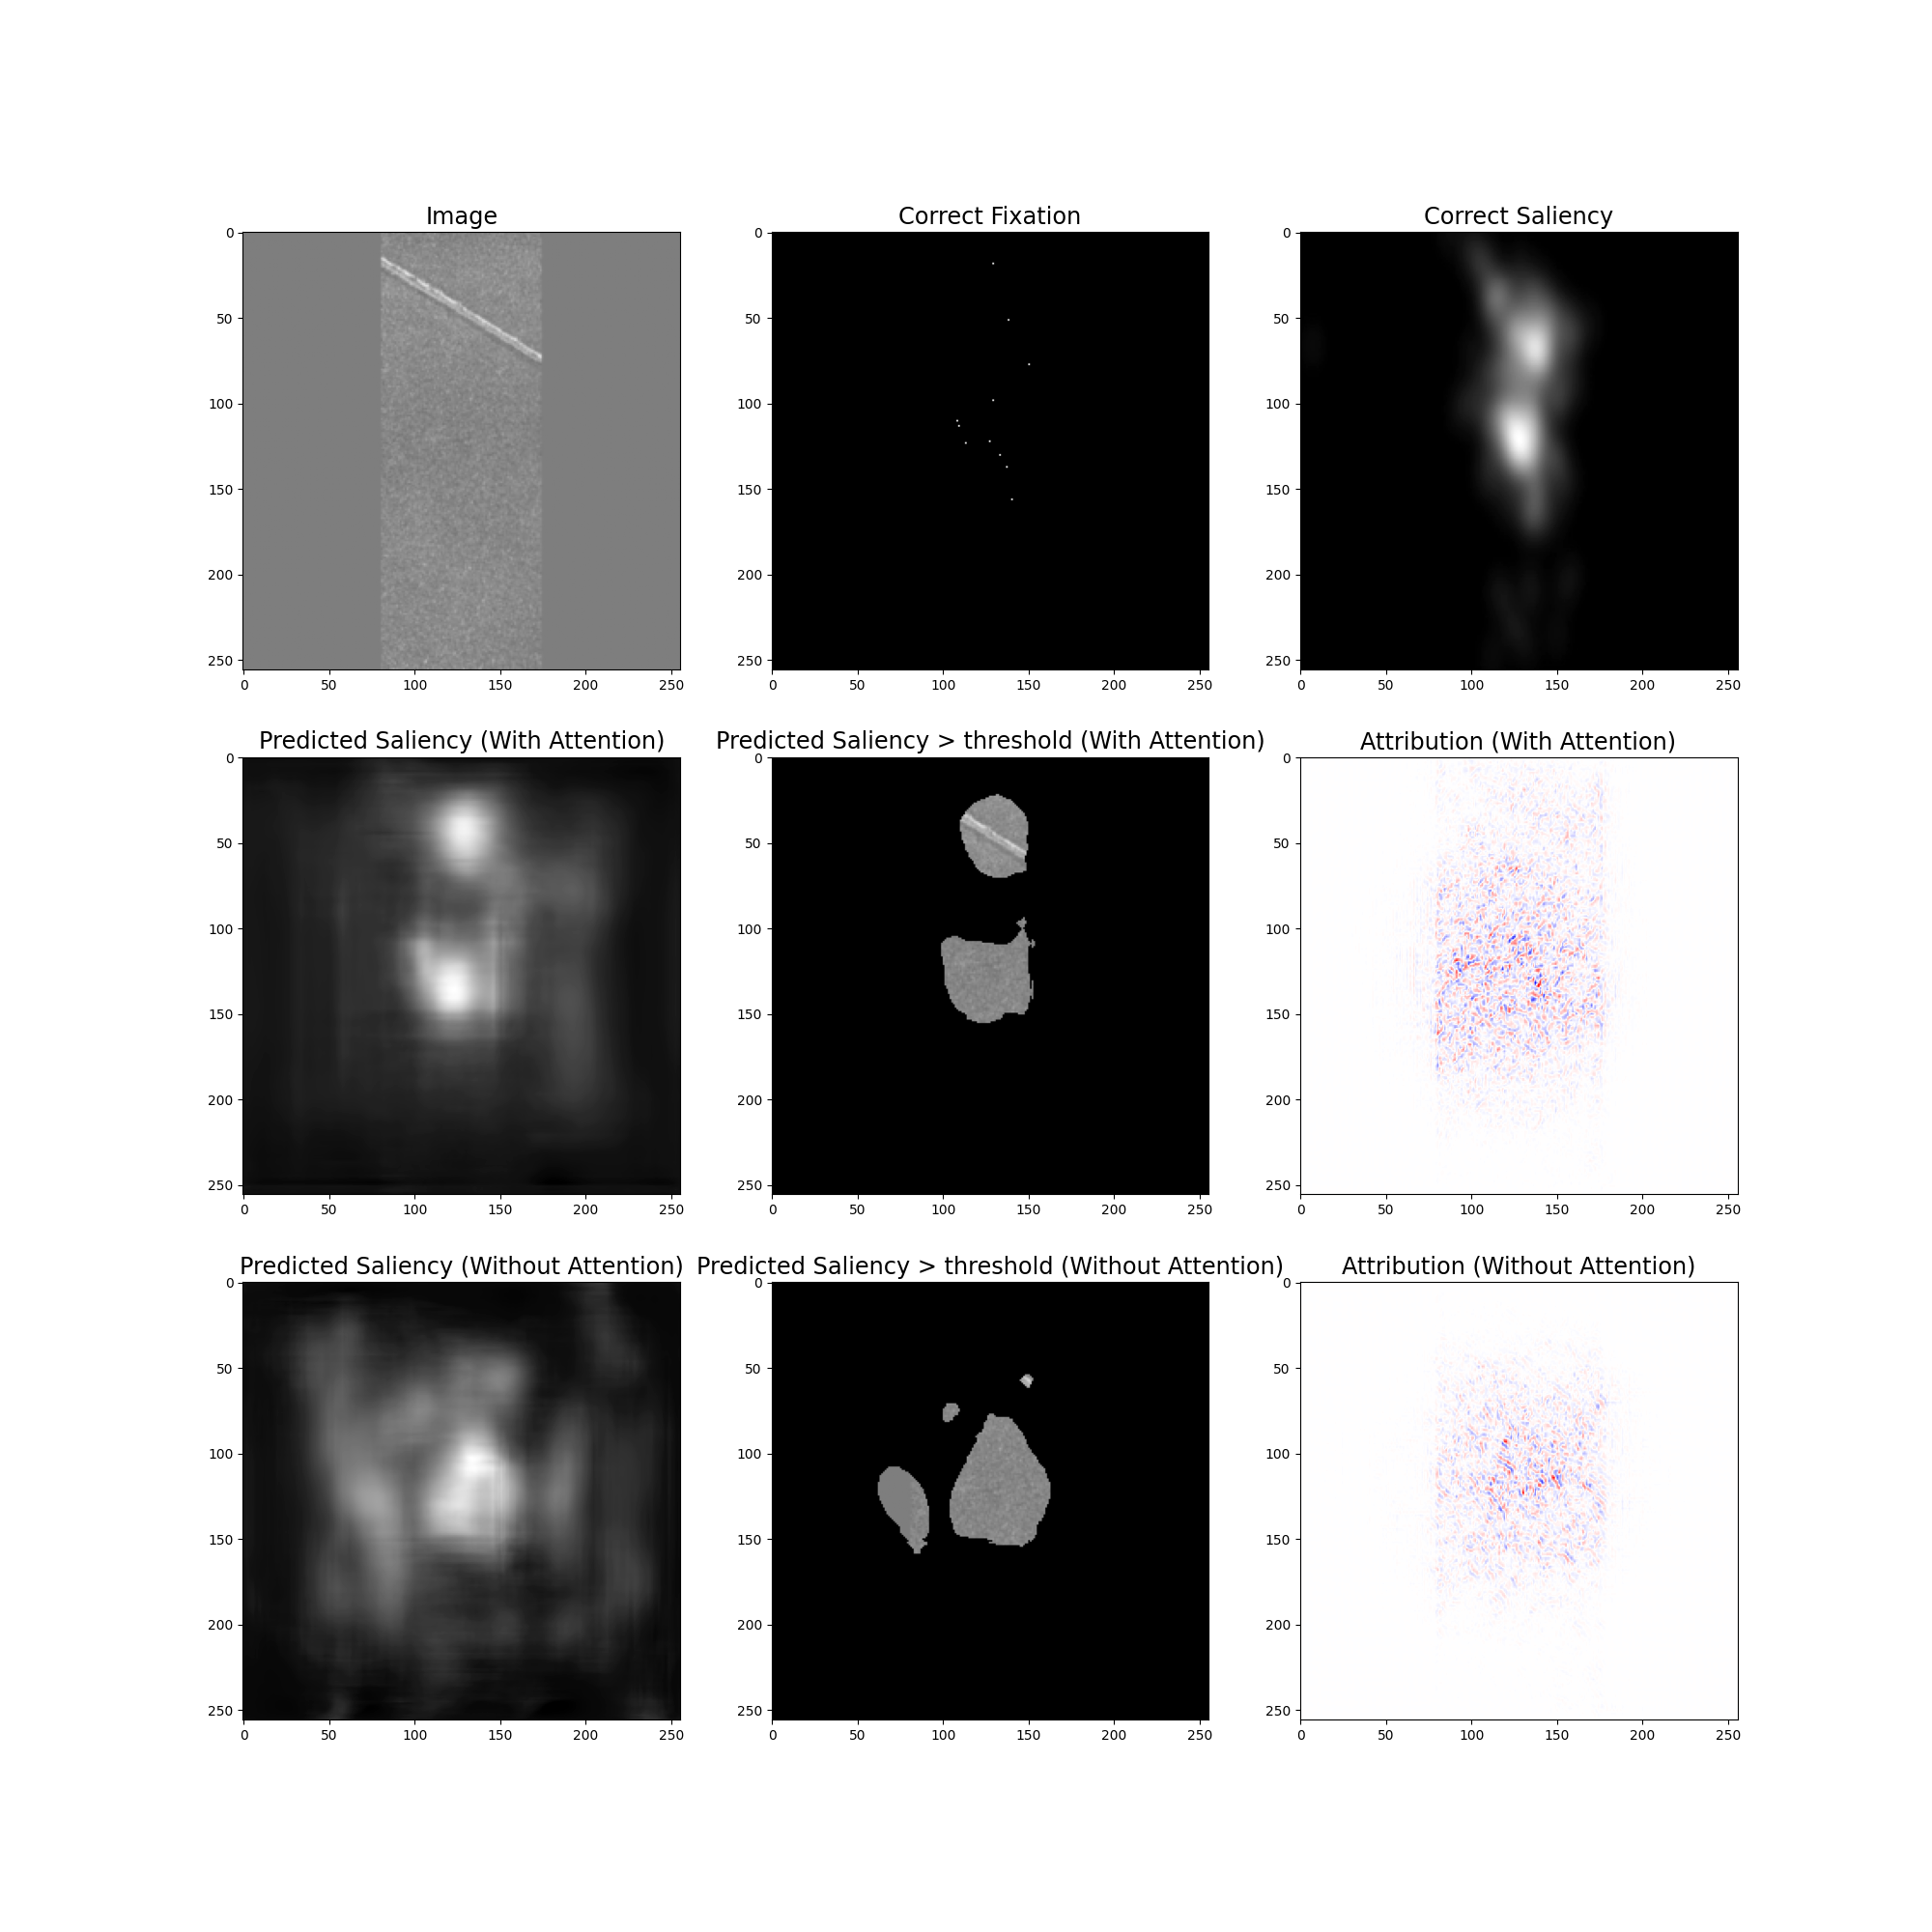
\includegraphics[width=7in]{imgs/used_example_2.png}
    \caption{A figure in Category ``Pattern'' of CAT2000, which is almost the same anywhere except a stick in a similar colour on the edge . The model with an attention layer fixes its attention in the middle of the figure while still finding the obscure stick.}
    \label{img:int_example_2}
\end{figure}

% % % Modified by Linsage: Add Verification and Interpretation end






\section{Discussion, Conclusions, Future work}
% % % Modified by Linsage: Add Discussion and Future Work begin
\subsection{Discussion}

In this project, we implement an attention layer and attach it to the traditional UNet to do saliency detection tasks.
We try different loss functions and metrics, but since the UNet is complicated enough, an attention layer with a simple structure cannot significantly improve the performance.
Despite this, we find that our model with the attention mechanism has better performance on some individual pictures.
We also implement the Integrated Gradients method to analyze the result of these pictures.
We find that the focused patterns themselves and some background or margin information strongly contribute to the result, which may help people make more conjectures about how surrounding patterns help decide saliency.
This makes us believe that global information is important in saliency detection tasks.



Although it is not a successful attempt, we conclude a few takeaway advice in model and dataset selection:
If we would verify the usage of a simple unit, we should also begin with a compatible size model.
We can also train and test on datasets with different distributions and characteristics to explore the limitations of models.

\subsection{Ethics}
The first ethical concern is data privacy. 
When the model is trained, figures derived by subjects’ eye movements are sent into the model, 
which carries some personal information. 
Although the parameters in the model store abstract features, 
there is still a concern that some particular patterns are recorded in the model,
mainly when we use an attention level that receives features of lower levels.
For example, if some parts of a figure attract a subject while other people will not pay attention to these parts,
the effect on the saliency map will not be conspicuous in the training data after averaging.
However, if the model boosts the weight of this particular information,
and some people compare the strange outputs with the actual data from other people,
they will know for sure that the model has some preference,
which can be derived from the eye movement data of one of the subjects.

The second issue is that our model may not produce a good representation of real data. 
SALICON dataset usually contains normal figures.
CAT2000 includes various abnormal types of figures, but probably they cannot perfectly imitate the distribution of information in the real world.
When we are playing games or watch slides, the information boxes,
the moving arrow of the mouse, and some other disturbance will explicitly influence human saliency detection.
If we design our compression algorithm depending totally on predicted saliency,
it will not always have good performance.
The subjects that contribute their eye movement data also cannot represent all the people in the world.
Children, people with color deficiency, or experts in some fields may have some special preference in their attention system.

The most harmful issue can be the misuse of the model. 
If saliency can be detected at a low price, the parameter can be tuned to do the opposite, 
which is detecting the areas that may attract the least attention. 
Some ill-disposed people will take advantage of this to hide some unhealthy or harmful contents in the most inconspicuous parts of the pictures to avoid being checked by supervisors. 
This can cause undetectable hurt to the users of these media files.

\subsection{Future Work}

If we have another semester to work on this project, we may try to optimize the network framework.
The purpose of saliency detection is efficiently processing the most useful information, and the attention layer we add acts as a gate to discard unimportant information in early processing to save computing resources.
We can try to modify the network like this: When the amount of information is big (at the beginning and the end of the network), we will make the computation simpler, namely constructing CNNs with fewer kernels and layers.
When the information is abstract (in the middle), we will decrease the number of neurons.
This kind of decreasing computing resources may force the network to transmit information more efficiently.
In this kind of network, we can also change the position of the attention layer to see which place is the most optimized to get an idea of how the early selection and late selection mechanisms are separated and cooperated in the human brain.

If people would like to continue working on this project, they may try to create a more abundant dataset. The CAT2000 has made a good start because it contains a considerable number of unconventional pictures.
Although these kinds of pictures are not normal, there is a high possibility that they can be seen in games, slides, and videos, which is more similar to the environment of human vision.
However, the distribution of pictures in the dataset does not accord with the human experience because we do not see indoor scenes and satellite maps at the same frequency.
Suppose there are some portable devices for recording eye movements. In that case, we can create a dataset directly based on human experience (privacy is also a problem), which can create a more generalized saliency detection model.
We can also include the brain imaging data in the dataset to help improve the network structure.


% % % Modified by Linsage: Add Discussion and Future Work end

\section{Task Distribution}
Credits for implementation:
\begin{itemize}
    \item training, validation and test procedure (Shupei)
    \item SALICON data handling (Shupei)
    \item CAT2000 data handling (Sijie)
    \item FIGRIM and Fillers data handling (Mehdi)
    \item loss functions: NSS, CC, shuffled AUC, AUC-Borji, and AUC-Judd (NSS and CC implemented by Shupei, all AUC methods implemented by Mehdi)
    \item attention mechanism module (Shupei)
    \item integrated gradients algorithm framework (Sijie).
\end{itemize}

Credits for experiment:
\begin{itemize}
    \item training (Shupei and Mehdi)
    \item testing (Shupei and Sijie)
    \item analysis (Sijie)
\end{itemize}

% needs update
Credits for this report:
\begin{itemize}
    \item introduction (Shupei)
    \item related work (Shupei)
    \item datasets (Shupei and Sijie)
    \item interpretability (Sijie and Shupei)
    \item algorithm (Shupei and Sijie)
    \item performance measurement (Shupei and Sijie)
    \item results (Sijie and Shupei)
    \item interpretation and verification (Sijie)
    \item discussion, conclusions, future work (Sijie)
\end{itemize}
Mehdi proofread and revised the whole document.

\newpage

\bibliographystyle{unsrt}
\bibliography{proposal}


\end{document}
